\section*{Graf dosažitelnosti}
\label{sec:reachability_graph}

\newcommand{\mO}   {1, 0, 1, 0, 1, 0, 1, 0, 0, 0, 0, 0, 0}
\newcommand{\mI}   {0, 0, 1, 0, 1, 0, 1, 0, 0, 0, 0, 1, 0}
\newcommand{\mII}  {0, 0, 1, 0, 1, 1, 1, 0, 0, 0, 0, 0, 0}
\newcommand{\mIII} {0, 0, 1, 0, 1, 0, 0, 1, 0, 1, 0, 1, 0}
\newcommand{\mIV}  {0, 0, 1, 0, 1, 0, 0, 0, 1, 0, 1, 1, 0}
\newcommand{\mV}   {0, 1, 1, 0, 0, 0, 0, 0, 1, 0, 1, 1, 0}
\newcommand{\mVI}  {0, 0, 1, 0, 1, 0, 0, 1, 1, 0, 0, 1, 0}
\newcommand{\mVII} {0, 0, 0, 0, 0, 0, 0, 0, 1, 0, 1, 1, 1}
\newcommand{\mVIII}{1, 0, 0, 0, 0, 0, 0, 0, 1, 0, 1, 0, 1}
\newcommand{\mIX}  {0, 0, 0, 0, 0, 1, 0, 0, 1, 0, 1, 0, 1}
\newcommand{\mX}   {0, 1, 0, 1, 0, 1, 0, 0, 1, 0, 1, 0, 0}
\newcommand{\mXI}  {0, 0, 1, 0, 1, 1, 0, 0, 1, 0, 1, 0, 0}
\newcommand{\mXII} {0, 1, 1, 0, 0, 1, 0, 0, 1, 0, 1, 0, 0}
\newcommand{\mXIII}{0, 0, 1, 0, 1, 1, 0, 1, 1, 0, 0, 0, 0}

Pro graf dosažitelnosti jsem zvolil verzi sítě (viz \figref{fig:network}) k-omezenou pro pouze 1 auto na křižovatce tedy $M_0$ = \orderArrayNumbered{\mO}.

\begin{figure}[h!]
    \centering
    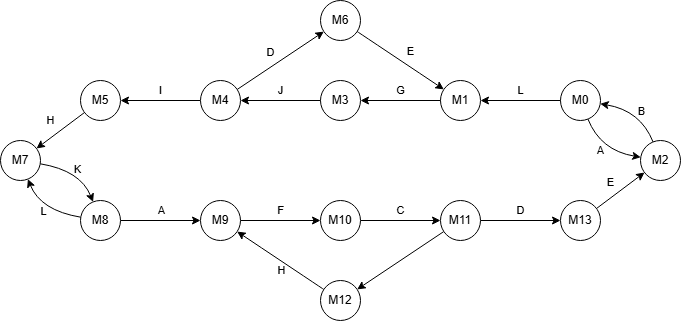
\includegraphics[width=1.0\textwidth]{assets/graphK1}
    \caption{Graf dosažitelnosti pro k-omezenou síť s jedním autem na křižovatce.}
    \label{fig:reachability_graph_k1}
\end{figure}

\newcommand{\convertArrayToColumn}[1]{%
    \av{\mO}{#1} & \av{\mI}{#1} & \av{\mII}{#1} & \av{\mIII}{#1} & \av{\mIV}{#1} & \av{\mV}{#1} & \av{\mVI}{#1} & \av{\mVII}{#1} & \av{\mVIII}{#1} & \av{\mIX}{#1} & \av{\mX}{#1} & \av{\mXI}{#1} & \av{\mXII}{#1} & \av{\mXIII}{#1}
}

\newcommand{\conn}[2]{%
    \overset{#1}{\xrightarrow{\hspace{0.2cm}}}M#2
}

\begin{table}[h!]
    \centering
    \resizebox{1.0\textwidth}{!}{
        \begin{tabular}{c|c|c|c|c|c|c|c|c|c|c|c|c|c|c}
                              & M0 & M1 & M2 & M3 & M4 & M5 & M6 & M7 & M8 & M9 & M10 & M11 & M12 & M13 \\
            \hline
            \textbf{$p_1$}    & \convertArrayToColumn{0} \\
            \textbf{$p_2$}    & \convertArrayToColumn{5} \\
            \textbf{$p_3$}    & \convertArrayToColumn{6} \\
            \textbf{$p_4$}    & \convertArrayToColumn{7} \\
            \textbf{$p_5$}    & \convertArrayToColumn{8} \\
            \textbf{$p_6$}    & \convertArrayToColumn{9} \\
            \textbf{$p_7$}    & \convertArrayToColumn{10} \\
            \textbf{$p_8$}    & \convertArrayToColumn{11} \\
            \textbf{$p_9$}    & \convertArrayToColumn{12} \\
            \textbf{$p_{10}$} & \convertArrayToColumn{1} \\
            \textbf{$p_{11}$} & \convertArrayToColumn{2} \\
            \textbf{$p_{12}$} & \convertArrayToColumn{3} \\
            \textbf{$p_{13}$} & \convertArrayToColumn{4} \\
            \hline
                              & \conn{A}{2} & \conn{G}{3} & \conn{B}{0} & \conn{J}{4} & \conn{D}{6} & \conn{H}{7} & \conn{E}{1} & \conn{K}{8} & \conn{A}{9} & \conn{F}{10} & \conn{C}{11} & \conn{L}{12} & \conn{H}{9} & \conn{E}{2} \\
                              & \conn{L}{1} &             &             &             & \conn{I}{5} &             &             &             &             &              &              & \conn{D}{13} &             &             \\
        \end{tabular}
    }
    \caption{Tabulka pro strom dosažitelnosti viditelný na \figref{fig:reachability_graph_k1}.}
    \label{tab:rereachability_transitions}
\end{table}

\newpage
\subsection*{K-omezení sítě pro více aut}
\label{subsec:more_cars}

Pro síť zobrazenou na \figref{fig:network} dochází s postupným zvyšováním maximálního počtu aut, která mohou být současně v křižovatce, k exponenciálnímu rozšiřování grafu dosažitelnosti.
Tento růst lze sledovat na \figref{fig:reachability_graph_k2} a \figref{fig:reachability_graph_k3}, kde se graf postupně stává natolik složitým, že jeho analýza je prakticky neproveditelná.

Navzdory tomuto faktu, je viditelné, že základní vlastnosti sítě zůstávají zachovány.
Jedinou změnou vlastnosti, je zamítnutí bezpečnosti sítě, která je podmíněna pravidlem, že každý stav musí nabývat maximálně jeden token.

\begin{figure}[h!]
    \centering
    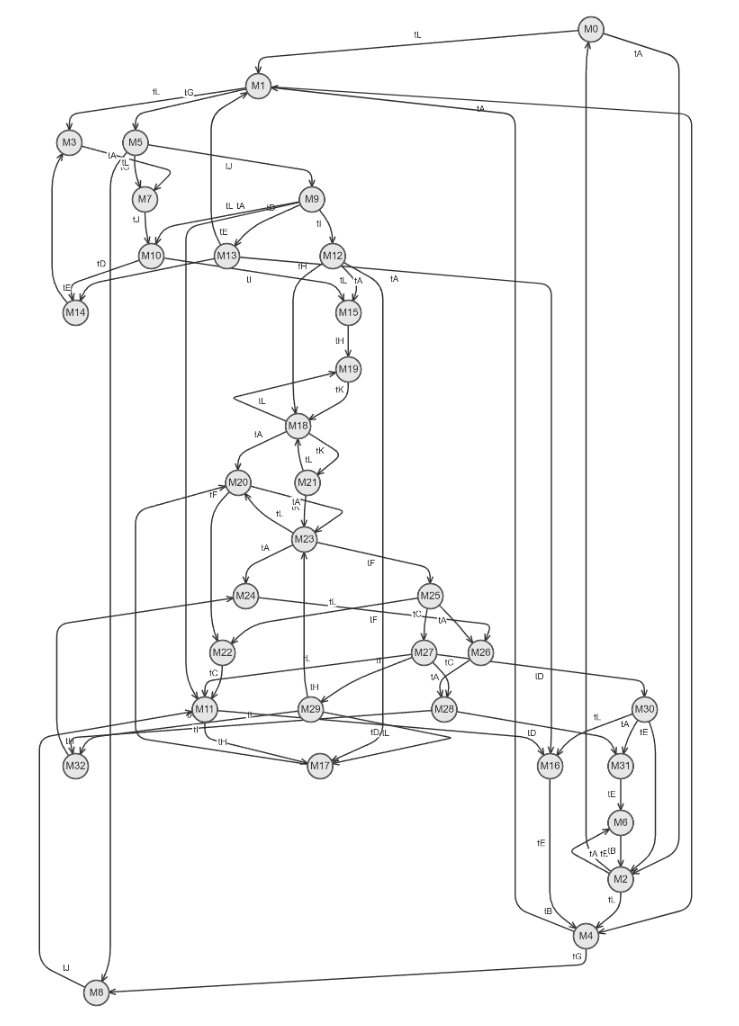
\includegraphics[width=0.8\textwidth]{assets/graphK2_auto}
    \caption{Graf dosažitelnosti pro k-omezenou síť s dvěma auty v křižovatce.}
    \label{fig:reachability_graph_k2}
\end{figure}

\begin{figure}[H!]
    \centering
    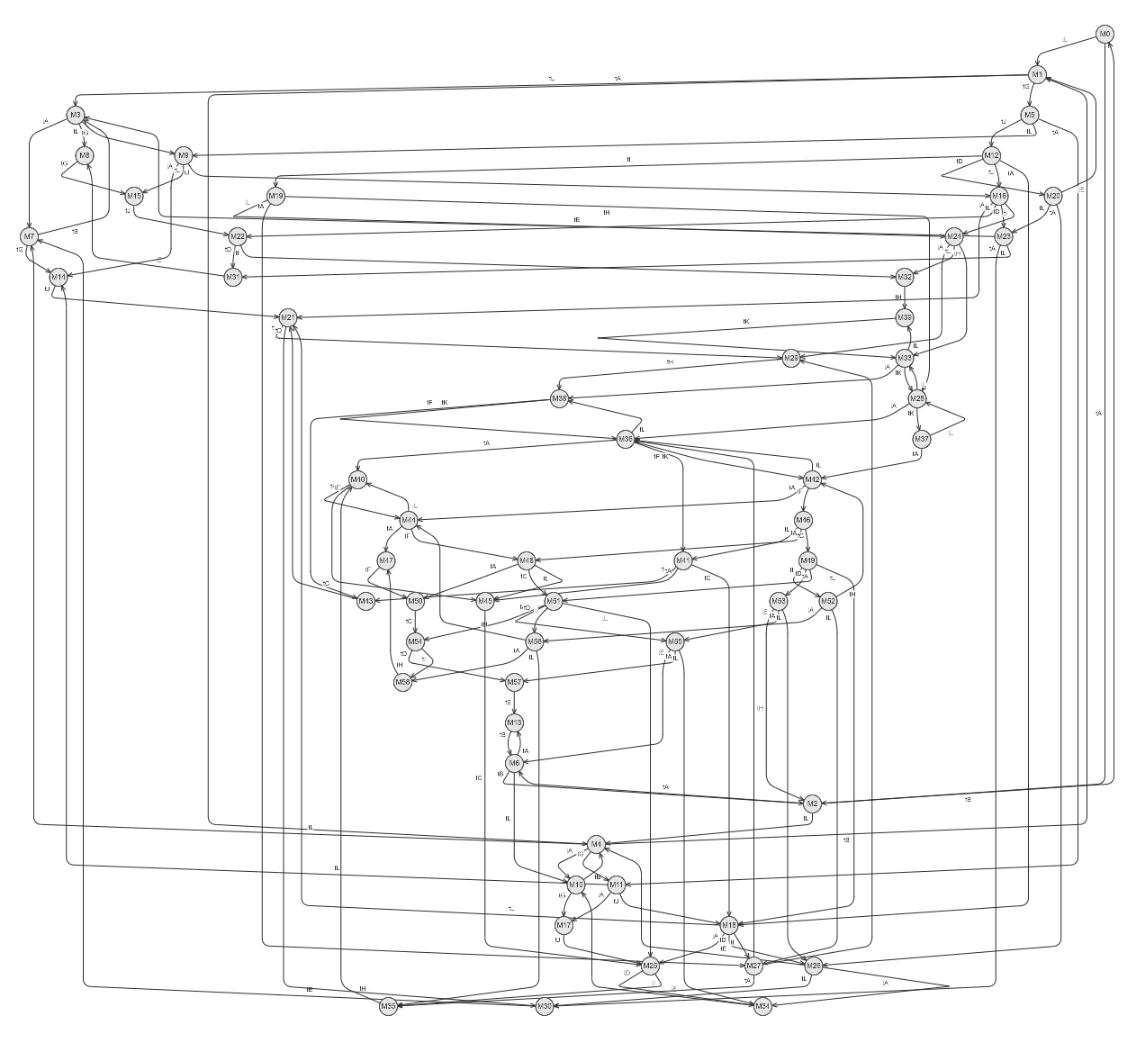
\includegraphics[width=1.0\textwidth]{assets/graphK3_auto}
    \caption{Graf dosažitelnosti pro k-omezenou síť s třemi auty v křižovatce.}
    \label{fig:reachability_graph_k3}
\end{figure}

\begin{table}[H!]
    \renewcommand{\arraystretch}{1.3}
    \resizebox{\textwidth}{!}{%
        \begin{tabular}{P{10cm}|P{10cm}}
            \textbf{Maximální počet aut v křižovatce} & \textbf{Počet dosažitelných značení} \\
            \hline
            1    & 13      \\
            2    & 32      \\
            3    & 58      \\
            4    & 91      \\
            5    & 131     \\
            10   & 218     \\
            $>$10 & $>$250 \\
        \end{tabular}%
    }
    \caption{Tabulku počtu dosažitelných značení pro k-omezenou síť s různým počtem aut v křižovatce.}
    \label{tab:reachability_count}
\end{table}

\FloatBarrier

\endinput